\chapter{RTL Design and Verification}
\label{chap:rtl_design}

The UART IP core was developed using Verilog HDL following a modular design methodology. The complete RTL design consists of four independent modules: the Baud Rate Generator, UART Transmitter, UART Receiver, and the UART Top module. Each module was verified individually using dedicated testbenches before performing complete system-level verification.

The RTL implementation was written to be fully synthesizable and compatible with the SkyWater SKY130 standard cell library used by the OpenLane2 ASIC design flow.

\vspace{0.3cm}

The verification process consisted of individual module simulations followed by complete UART functionality testing.

%%%%%%%%%%%%%%%%%%%%%%%%%%%%%%%%%%%%%%%%%%%%%%%%%%%%%%%%%%%%

\section{RTL Module Organization}

The complete UART design is divided into four reusable RTL modules.

\begin{table}[!htbp]
\centering
\caption{UART RTL modules}
\label{tab:rtl_modules}
\begin{tabular}{ll}
\toprule
Module & Function\\
\midrule
Baud Generator & Generates baud tick from system clock\\
UART Transmitter & Converts parallel data into serial data\\
UART Receiver & Converts serial data into parallel data\\
UART Top & Integrates all UART modules\\
\bottomrule
\end{tabular}
\end{table}

The modular architecture improves readability, verification, scalability and future reuse of the IP.

%%%%%%%%%%%%%%%%%%%%%%%%%%%%%%%%%%%%%%%%%%%%%%%%%%%%%%%%%%%%

\section{Baud Rate Generator}

The baud rate generator produces a periodic \texttt{baud\_tick} signal required by both the transmitter and receiver. It divides the incoming system clock using a programmable counter so that data transmission occurs at the required baud rate.

\subsection*{Module Interface}

\begin{table}[!htbp]
\centering
\caption{Baud Generator ports}
\label{tab:baud_ports}
\begin{tabular}{llll}
\toprule
Signal & Direction & Width & Description\\
\midrule
clk & Input & 1 & System clock\\
rst & Input & 1 & Active-high reset\\
baud\_tick & Output & 1 & Baud timing pulse\\
\bottomrule
\end{tabular}
\end{table}

The RTL schematic generated by Yosys is shown below.

\begin{figure}[!htbp]
\centering
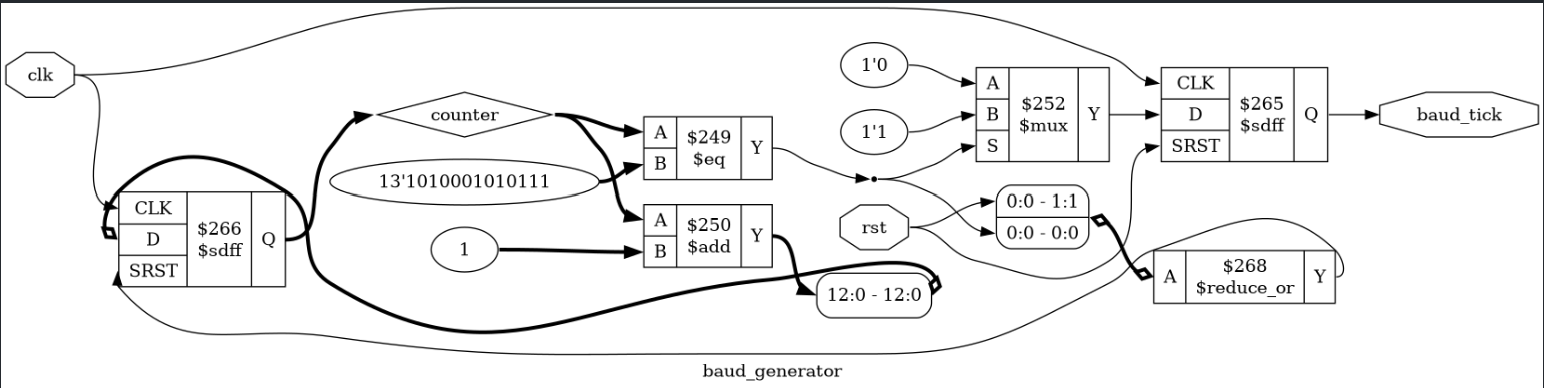
\includegraphics[width=\textwidth]{images/baud_generator_rtl.png}
\caption{RTL schematic of the Baud Rate Generator generated using Yosys.}
\label{fig:baud_rtl}
\end{figure}

%%%%%%%%%%%%%%%%%%%%%%%%%%%%%%%%%%%%%%%%%%%%%%%%%%%%%%%%%%%%

\section{UART Transmitter}

The transmitter converts an 8-bit parallel word into a serial UART frame consisting of a start bit, eight data bits and a stop bit. Data shifting is synchronized using the baud tick generated by the baud rate generator.


\subsection*{Module Interface}

\begin{table}[!htbp]
\centering
\caption{UART transmitter ports}
\label{tab:tx_ports}
\begin{tabular}{llll}
\toprule
Signal & Direction & Width & Description\\
\midrule
clk & Input & 1 & System clock\\
rst & Input & 1 & Reset\\
baud\_tick & Input & 1 & Baud timing pulse\\
tx\_start & Input & 1 & Transmission enable\\
tx\_data & Input & 8 & Parallel input data\\
tx & Output & 1 & Serial output\\
tx\_busy & Output & 1 & Busy flag\\
\bottomrule
\end{tabular}
\end{table}

\begin{figure}[!htbp]
\centering
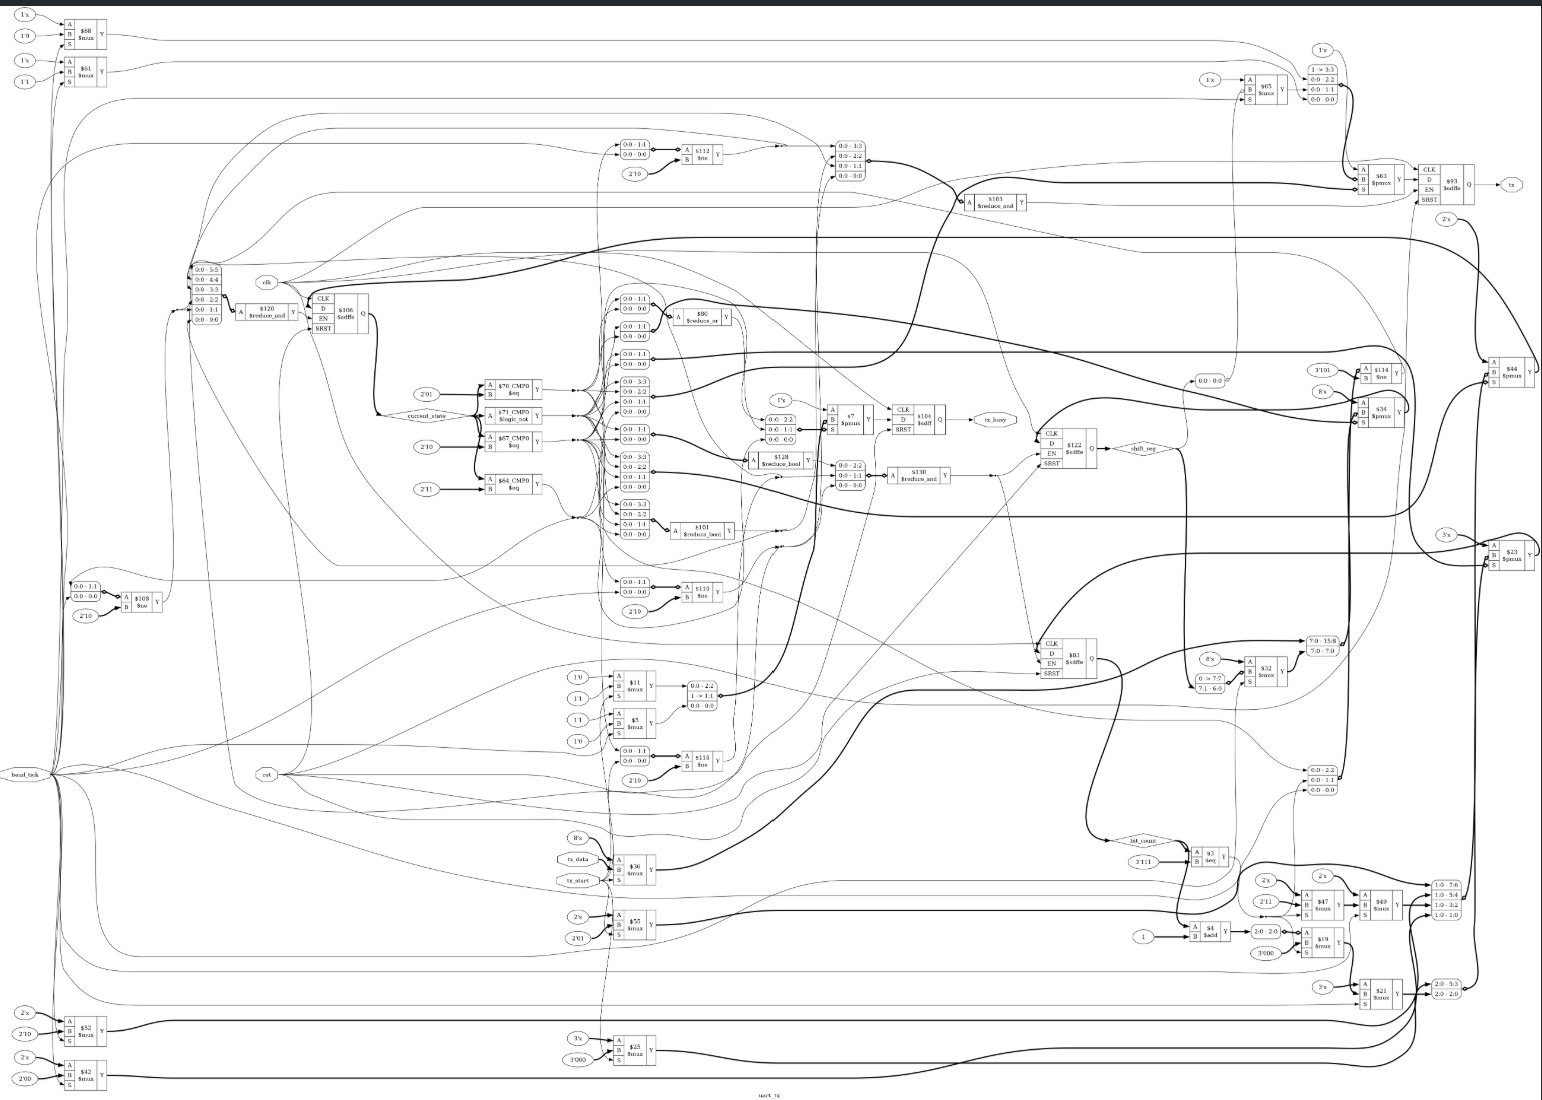
\includegraphics[width=\textwidth]{images/uart_tx_rtl.png}
\caption{RTL schematic of the UART transmitter generated using Yosys.}
\label{fig:tx_rtl}
\end{figure}

%%%%%%%%%%%%%%%%%%%%%%%%%%%%%%%%%%%%%%%%%%%%%%%%%%%%%%%%%%%%

\section{UART Receiver}

The receiver continuously monitors the RX line for a valid start bit. After detecting the start bit, it samples each incoming data bit at the baud rate and reconstructs the original 8-bit data word.


\subsection*{Module Interface}

\begin{table}[!htbp]
\centering
\caption{UART receiver ports}
\label{tab:rx_ports}
\begin{tabular}{llll}
\toprule
Signal & Direction & Width & Description\\
\midrule
clk & Input & 1 & System clock\\
rst & Input & 1 & Reset\\
baud\_tick & Input & 1 & Baud timing pulse\\
rx & Input & 1 & Serial input\\
rx\_data & Output & 8 & Received data\\
rx\_done & Output & 1 & Reception complete flag\\
\bottomrule
\end{tabular}
\end{table}

\begin{figure}[!htbp]
\centering
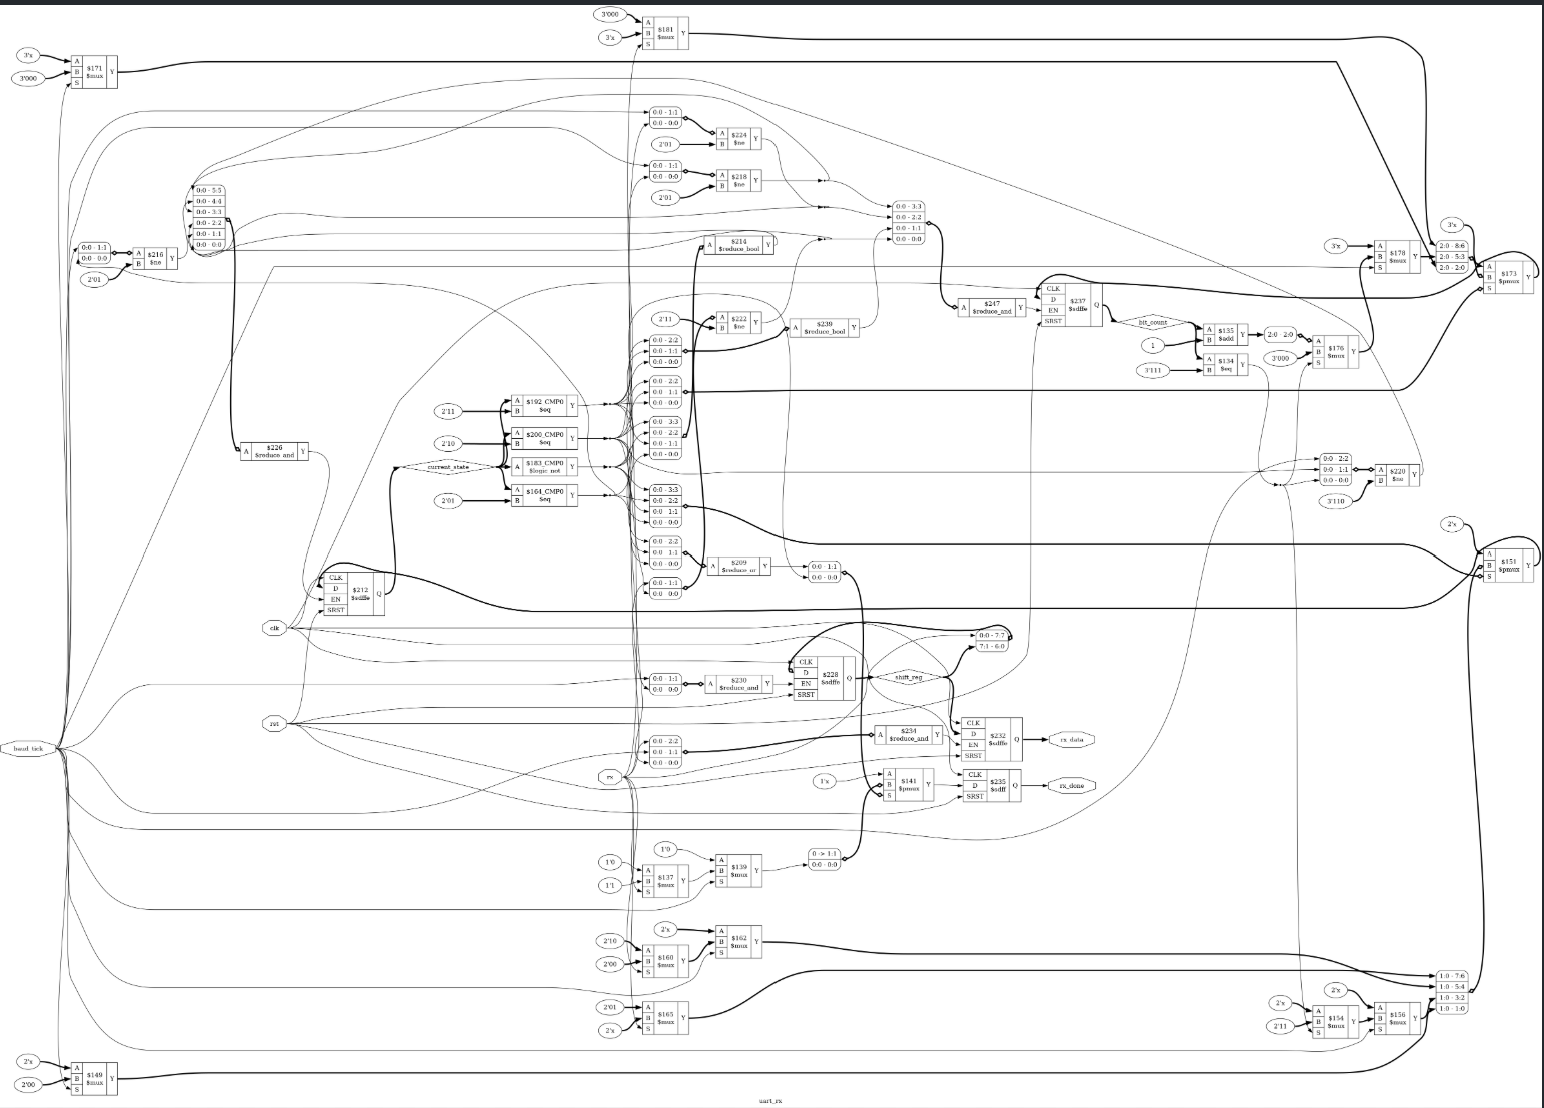
\includegraphics[width=\textwidth]{images/uart_rx_rtl.png}
\caption{RTL schematic of the UART receiver generated using Yosys.}
\label{fig:rx_rtl}
\end{figure}

%%%%%%%%%%%%%%%%%%%%%%%%%%%%%%%%%%%%%%%%%%%%%%%%%%%%%%%%%%%%

\section{UART Top Module}

The UART top module integrates the baud generator, transmitter and receiver into a complete UART IP core. The baud tick generated by the baud generator is shared by both transmitter and receiver to ensure synchronized operation.


\begin{figure}[!htbp]
\centering
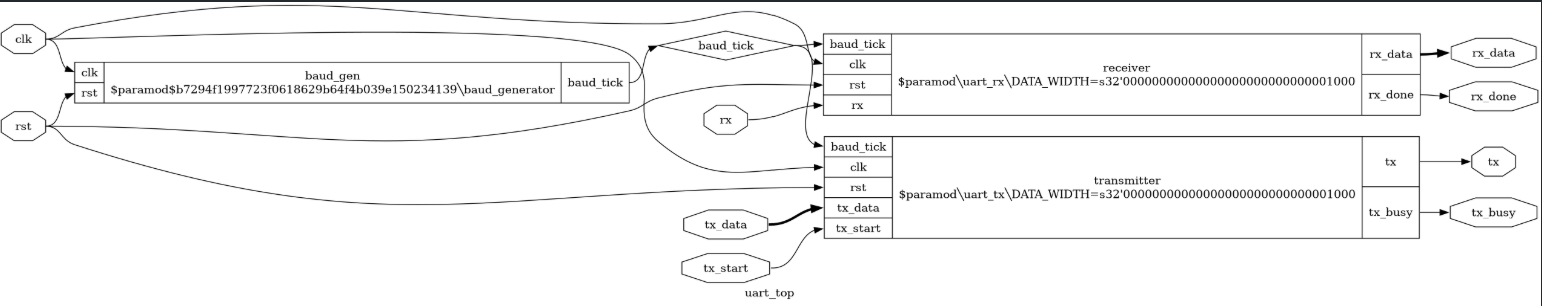
\includegraphics[width=\textwidth]{images/uart_top.png}
\caption{RTL hierarchy of the complete UART top module generated using Yosys.}
\label{fig:top_rtl}
\end{figure}

%%%%%%%%%%%%%%%%%%%%%%%%%%%%%%%%%%%%%%%%%%%%%%%%%%%%%%%%%%%%

\section{Functional Verification}

Each RTL module was verified independently using dedicated Verilog testbenches. After successful individual verification, the complete UART IP core was simulated to validate end-to-end serial communication.

The functional verification confirmed:

\begin{itemize}
\item Correct baud tick generation.
\item Proper UART frame transmission.
\item Accurate serial-to-parallel data reception.
\item Successful integration of transmitter, receiver and baud generator.
\end{itemize}

The simulation waveforms are presented in Chapter~\ref{chap:results}, where the functional behavior of each module is analyzed in detail.